\section{Tecnologia Utilizzata}
In questa sezione verranno illustrate le tecnologie utilizzate per la realizzazione dell'elaborato
\subsection{NDEF e Sicurezza}
\hspace{\parindent}NDEF è un preciso standard per un formato di dati sui chip NFC, viene utilizzato in applicazioni quali le carde di credito, o gli smart poster, la struttura di un messaggio è quella vista nella seguente figura: 
\begin{figure}[h]
\begin{center}
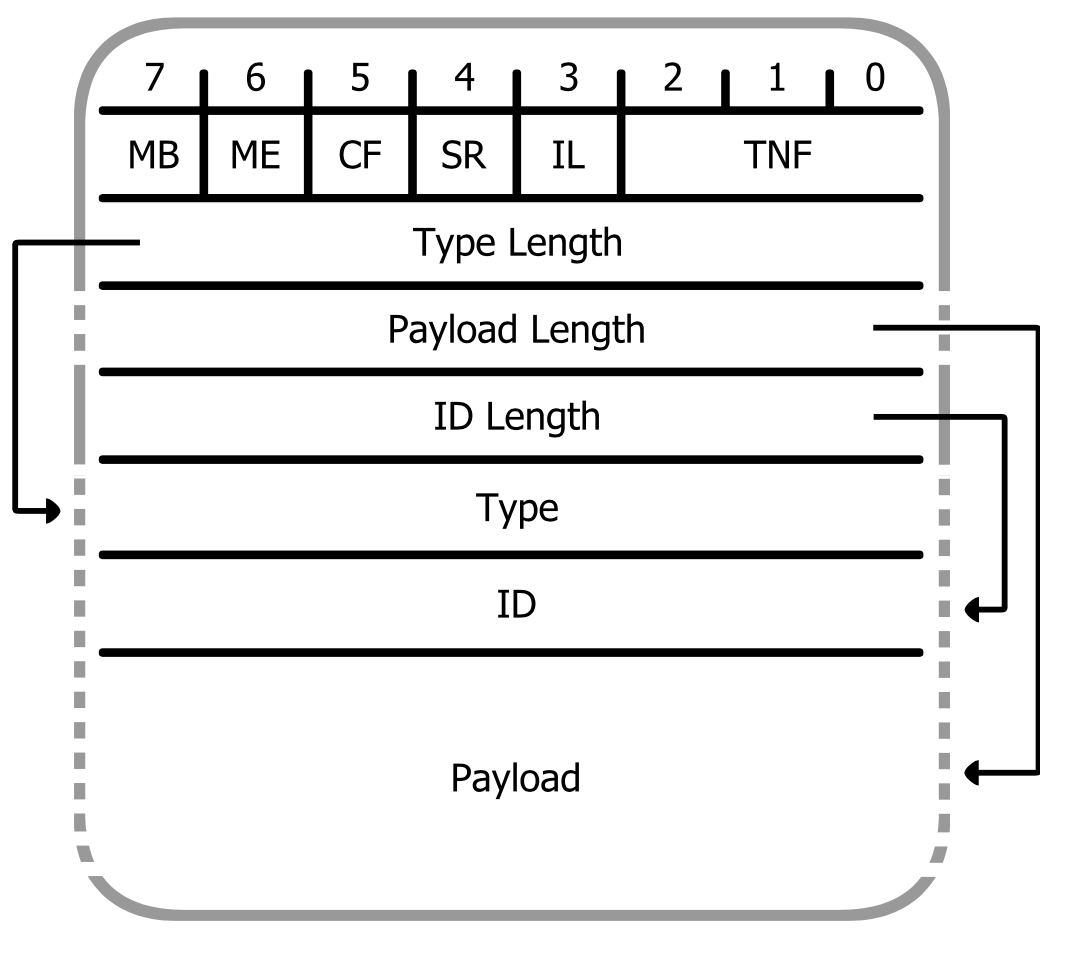
\includegraphics[scale=0.45]{ndefstructure}
\caption[NDEF Vulnerabilità]{Vulnerabilità NDEF\footnotemark}
\end{center}
\end{figure}
\footnotetext{\url{www.researchgate.net/publication/224227216_Security_Vulnerabilities_of_the_NDEF_Signature_Record_Type}}
In ordine abbiamo: 
\paragraph{Header}
Che è composto da: Message Begin (MB), Message End (ME), Chunk Flag (CF), Short record (SR), ID Length present (IL), Type Name Format (TNF), Length fields, Type, ID
\\I primi 5 parametri sono dei flag, per finire invece abbiamo il \textbf{Payload} che è il messaggio.
\\Detto questo andiamo a concentrarci meglio su determinati campi quindi:
\paragraph{•}CF: indica il record che fa parte di una catena di record, quando il suo valore è pari a 1 vuol dire che c'è \textit{almeno} 1 altro record nella catena, invece quando non è settato vuol dire che ci troviamo o nel caso di record singolo o nel caso di ultimo elemento della catena. Una cosa da notare è che ME e CF non possono essere entrambi settati a 1
\paragraph{•}SR: quando viene messo ad 1 vuol dire che il record corrente è di tipologia short, questo comporta che il campo Payload Length, che si trova dentro Length fields, viene espresso tramite 1 byte, in alternativa viene espresso da 4 byte
\paragraph{•} IL: indica se nel record è presente un identificatore, se non dovesse essere abilitato questo comporta che non vi saranno il campo ID Length e il campo ID che è quello di identificazione del record.
\paragraph{•}TNF: serve per indicare la struttura del campo Type, è composto da 3 bit e può assumere solo i valori da 0 a 6 perché il numero 7 è riservato.
\\\\NDEF ha anche una firma
\begin{figure}[h]
\begin{center}
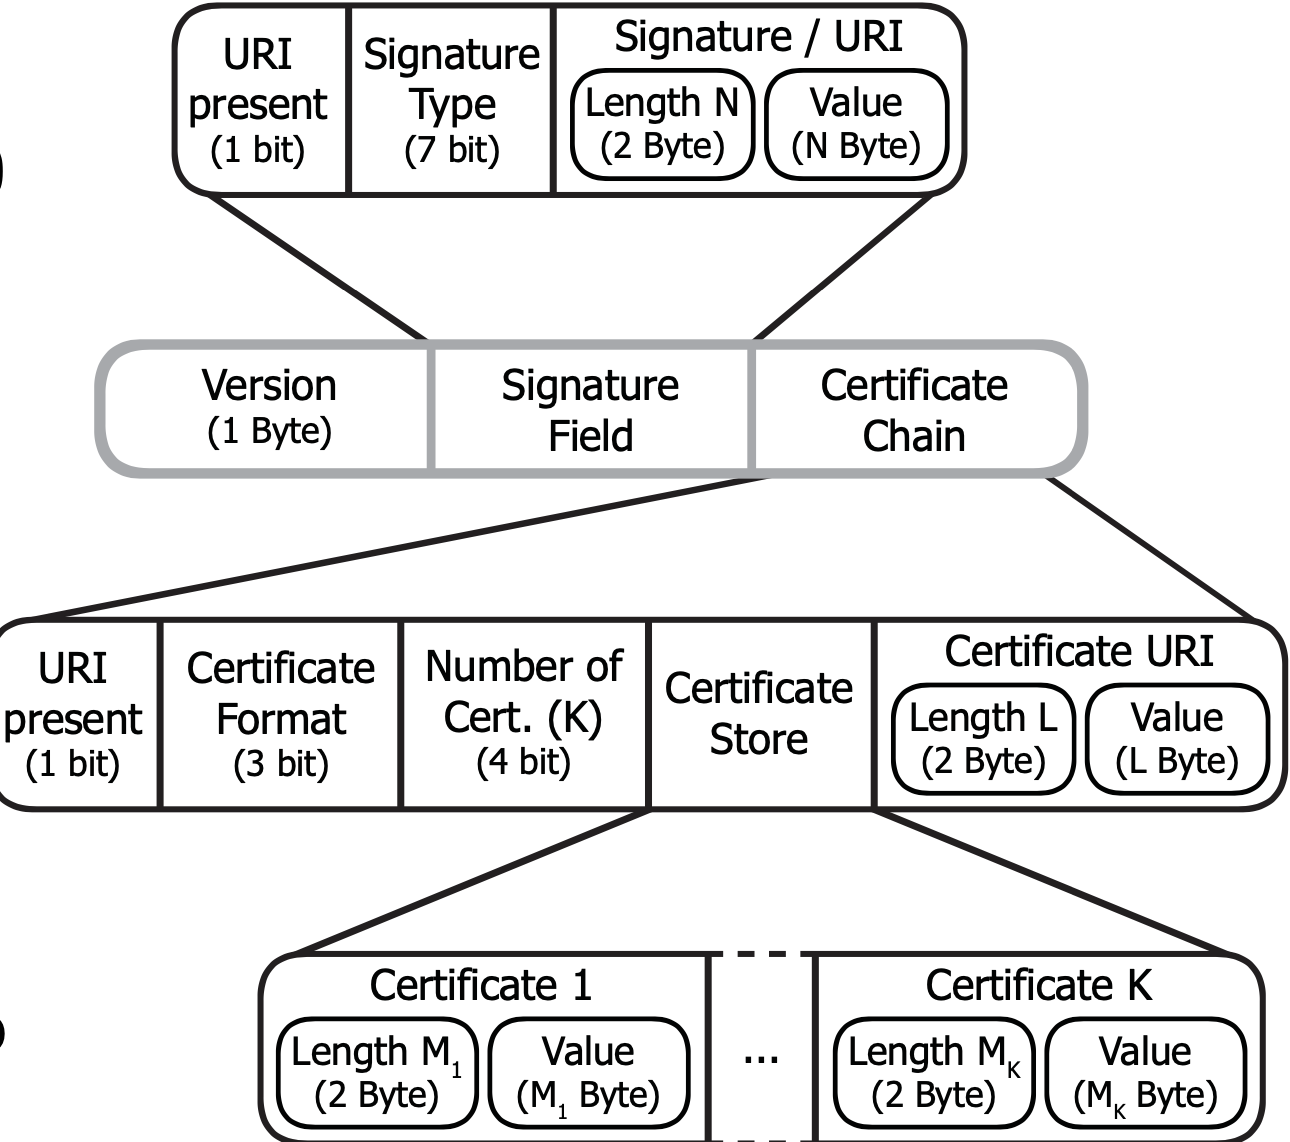
\includegraphics[scale=0.6]{ndefsign}
\caption[NDEF Vulnerabilità]{Vulnerabilità NDEF\footnotemark}
\end{center}
\end{figure}
\footnotetext{\url{www.researchgate.net/publication/224227216_Security_Vulnerabilities_of_the_NDEF_Signature_Record_Type}}
\\L'ultimo documento di specifica è stato rilasciato nel Novembre 2010, sostanzialmente ha una struttura fatta da un \textbf{campo firma}, che può essere una firma o una referenza URI ad una firma e da una \textbf{catena di certificati}, che è una catena di certificati PKI su un percorso sicuro.
\\Il record con la firma viene aggiunto ad una sequenza di record, e questo firma ogni record tra il record di firma appena precedente e se stesso, infatti un messaggio NDEF può contenere più di una firma.
\subsubsection{Cosa viene firmato?}
\hspace{\parindent} I campi che non vengono firmati sono MB/ME, questo perché se venissero firmati la firma non potrebbe essere agganciata al messaggio NDEF già firmato. Type, ID e Payload invece vanno firmati per assicurare l'integrità dei dati, mentre quando TNF viene cambiato, l'intero significato del record cambia, può essere quindi usato per nascondere dei record (identificati da type "Unknown"). 
\subsubsection{Sicurezza}
\hspace{\parindent}La tecnologia NFC è un'evoluzione dell'RFID, da un lato risulta meno predisposta ad attacchi esterni ma dall'altro lato è soggetta alle problematiche di sicurezza del suo predecessore. Le possibili minacce di sicurezza a cui sono sottoposti sono quelle riguardanti l'acquisizione, o l'alterazione dei dati contenuti nel tag, queste minacce possono avvenire mediante interrogazioni fraudolente o mediante l'intercettazione delle informazioni mediante ricevitori radio durante la lettura da parte di un lettore autorizzato.
\subsubsection{Intercettazioni}
\hspace{\parindent}Nell'ambito dell'NFC ma soprattutto in maniera generale, nel campo delle comunicazioni wireless l'intercettazione dei dati è uno degli attacchi più comuni. Per effettuare quest'attacco serve attrezzatura progettata ad hoc, quindi antenne e lettori fatti su misura. Per quanto riguarda il caso specifico NFC è un attacco molto difficile da realizzare a causa sei seguenti fattori:
\paragraph{i} potenza emessa dallo strumento sotto intercettazione
\paragraph{ii} fattori ambientali
\paragraph{iii} presenza della crittografia

Quindi da questo capiamo che anche in base al tipo di tag \footnote{cap 2 par 2.3.1} un attacco può essere più facile o più difficile, per esempio un attacco su un tag di tipo 1 sarà molto più semplice che su un tag di tipo 4.
\\Ci sono anche contromisure come per esempio quella di diminuire il campo magnetico, magari aumentando il fattore di direzionalità delle antenne, oppure usare algoritmi di cifratura per il messaggio, algoritmi per esempio AES.
\subsubsection{Modifica dei dati}
\hspace{\parindent}La modifica dei dati è un problema molto pericoloso, questo perché risulta trasparente all'utente, ha come scopo quello di modificare i dati trasmessi e renderli "validi". Fortunatamente risulta un attacco molto difficile da eseguire perché bisognerebbe riuscire ad intercettare completamente ogni bit del messaggio e rimandarlo sulle frequenze precise, quindi ogni volta modulando il campo delle frequenze in modo specifico e diverso.
\subsubsection{Man in the middle}
\hspace{\parindent}È uno degli attacchi più pericolosi, infatti può arrecare molti danni ai sistemi coinvolti. Mentre sysA e sysB stanno comunicando, sysH, il dispisitivo dell'hacker, si interpone tra di loro. Durante la comunicazione sysH altera il dialogo che hanno sysA e sysB, mettendosi in mezzo e fingendosi sysA per sysB e sysB per sysA. La soluzione a questo attacco è quella di instaurare un canale sicuro, quindi usando una chiave per criptare i dati. 
Potrebbe succede che sysH cerchi di negoziare una chiave ai due sistemi però è molto complesso perché richiederebbe la visibilità di sysH.

\subsection{NoSQL Database}
\hspace{\parindent} I database NoSQL (non relazionali), sono realizzati per modelli di dati specifici, hanno degli schemi flessibili, un'ottima facilità di sviluppo, una scalabilità orizzontale e delle prestazioni ottime. Si può pensare all'attuale diffusione dei sistemi cloud, quindi una diffusione dove ci sono moltissimi nodi e usare un RDMBS (database relazionale) in questi casi diventerebbe molto difficile. I principali metodi d'implementazione dei database NoSQL sono:
\paragraph{•}Chiave-valore: I dati sono immagazzinati in un elemento che contiene una chiave oltre che i dati veri e propri, dal punto di vista implementativo questo è il metodo più semplice, però è anche quello meno efficiente nel caso nel quale le operazioni riguardano solo una parte dell'elemento e non l'elemento nel totale 
\paragraph{•}Column family: i dati vengono organizzati in righe e colonne, non si ha il bisogno di definire il numero di colonne e una riga può avere molte colonne
\paragraph{•}Document store: è un'evoluzione del metodo chiave-valore, i dati vengono salvati in un documento che può contenere un numero "infinito" di campi di "infinita" lunghezza, in questo modo riusciamo ad evitare sprechi di campi inutilizzati che andrebbero ad occupare spazio in memoria.

\subsection{WindowBuilder}
\hspace{\parindent}Per la realizzazione dell'interfaccia grafica in Java è stato usato il plug-in WindowBuilder di Eclipse. Questo plug-in è composto a partire dalle liberire SWT Designer e Swing Designer e rende comoda e veloce la creazione di interfacce grafiche (GUI) per le applicazioni Java. Usando il WYSIWYG visual designer e gli strumenti di layout è possibile creare finestre complesse, e per ogni elemento messo verrà generato il codice contente la posizione dell'elemento e la sua dichiarazione.
\\Inoltre, il codice generato da questa libreria non richiede l'uso di altre librerie personalizzate per compilarlo ed eseguirlo, inoltre è possibile dall'interfaccia grafica creare eventi che poi andranno compilati mediante codice scritto in dei blocchi di \textit{ActionListener}, è possibile generare diversi tipi di eventi, dal click del mouse, alla pressione di un tasto sulla tastiera, o persino al movimento nella finestra del mouse.

\subsection{Cassandra}
\hspace{\parindent}Apache Cassandra è un DBMS distribuito e open source. Si tratta di un progetto Top-Level, sviluppato da Apache Software Foundation per gestire grandi quantità di dati dislocati in diversi server, fornendo un servizio orientato alla disponibilità.
\\È una soluzione NoSQL che inizialmente fu sviluppata da Facebook, un modello di dati simile a BigTable in esecuzione su un'infrastruttura tipi Amazon-Dynamo. Cassandra fornisce una struttura di memorizzazione chiave-valore, con Eventual Consistency.
\subsubsection{CQLSH}
Reference\footnote{http://cassandra.apache.org/doc/latest/tools/cqlsh.html}
\begin{center}

\includegraphics[scale=0.15]{cassandra}
\end{center}
Alle chiavi corrispondono dei valori, raggruppati in famiglie di colonne: una famiglia di colonne è definita quando il database viene creato. Tuttavia le colonne possono essere aggiunte a una famiglia in qualsiasi momento.
\\Le colonne sono aggiunte solo specificando le chiavi, così differenti chiavi possono avere differenti numeri di colonne in una data famiglia. I valori di una famiglia di colonne sono memorizzati insieme, questo perché Cassandra adotta un approccio ibrido tra DBMS orientato alle colonne e la memorizzazione orientata alle righe.
\\Come caratteristiche principali abbiamo:
\paragraph{•} Fault-tolerance: i dati vengono replicati in maniera automatica su più nodi, la replica è supportata tramite vari data center e la sostituzione dei nodi può avvenire senza downtime\footnote{la replicazione verrà trattata nel capitolo 4.2}.
\paragraph{•} Tunable consistency: il livello di coerenza può essere modificato (da writes never fail a block for all replicas to be readable).

\subsection{UUID}
\hspace{\parindent}Un UUID\footnote{https://tools.ietf.org/html/rfc4122} conosciuto anche come Universally Unique Identifier, è un numero di 128 bit utilizzato per identificare informazioni nei sistemi informatici, lo si può trovare nell'rfc 4122.
\subsubsection{Come è formato?}
Il codice è composto da 16 byte, solitamente viene identificato da 32 caratteri esadecimali, a livello di sicurezza assume $ 3 \cdot 10^{38}$ possibili combinazioni
\begin{center}
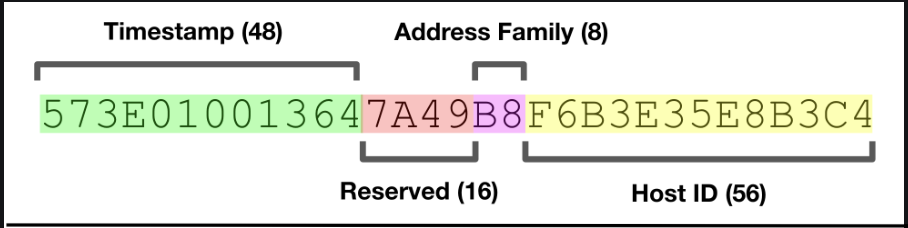
\includegraphics[scale=0.5]{uuid}
\end{center}
A differenza di altri sistemi l'unicità del codice generato non dipende da un'autorità centrale di registrazione o dal coordinamento delle parti che lo generano, però la sua probabilità di essere duplicato è talmente vicina a zero che viene considerata trascurabile.

\subsubsection{Analisi a livello matematico}

Considerando i 128 bit dell'UUID versione 4, 6 bit vengono riservati, quattro per la versione e due per altri parametri, quindi un UUID generato randomicamente ha 122 bit casuali. La probabilità che due UUID hanno lo stesso valore può essere calcolata usando la teoria delle probabilità (Paradosso del compleanno \footnote{https://betterexplained.com/articles/understanding-the-birthday-paradox/}). Usando quindi quest'approssimazione possiamo calcolare:
\begin{equation}
p(n) \approx 1- e^{-\frac{n^2}{2\cdot 2^x}}
\end{equation}
Notiamo quindi che quando il termine $ \frac{n^2}{2\cdot 2^x}$ è vicino allo zero, la probabilità può essere direttamente approssimata in questo modo:
\begin{equation}
p(n) \approx \frac{n^2}{2\cdot 2^x}
\end{equation}
Analizzandolo quindi in modo numerico potremo pensare che anche generando 1 miliardo di UUID ogni secondo per i prossimi 100 anni la probabilità di creare almeno un duplicato sarebbe circa del 50\%.

\subsection{Crittografia}